% Homework report template for courses lectured by Blaz Zupan.
% For more on LaTeX please consult its documentation pages, or
% read tutorials like http://tobi.oetiker.ch/lshort/lshort.pdf.
%
% Use pdflatex to produce a PDF of a report.

\documentclass[a4paper,11pt]{article}
\usepackage{a4wide}
\usepackage{fullpage}
\usepackage[utf8x]{inputenc}
\usepackage[toc,page]{appendix}
\usepackage[pdftex]{graphicx} % for figures
\usepackage{setspace}
\usepackage{color}
\definecolor{light-gray}{gray}{0.95}
\usepackage{listings} % for inclusion of Python code
\usepackage{hyperref}
\renewcommand{\baselinestretch}{1.2}

\lstset{ % style for Python code, improve if needed
language=Python,
basicstyle=\footnotesize,
basicstyle=\ttfamily\footnotesize\setstretch{1},
backgroundcolor=\color{light-gray},
}

\title{Homework \#3: Evolutionary Tree}
\author{Anže Pečar (63060257)}
\date{\today}

\begin{document}

\maketitle

\section{Introduction}

In the third homework we compare COX3 mitochindrial gene between multiple species and then build an evolutionary tree.

\section{Data}

Data was obtained from GenBank. We downloaded mitochondrial refrence sequences (RefSeq) for Canis lupus familiaris, Carassius auratus auratus, Chamaeleo calyptratus, Daboia russellii, Delphinus capensis, Equus caballus, Gorilla gorilla, Homo sapiens, Homo sapiens neanderthalensis, Pan troglodytes, Pongo abelii, Rattus norvegicus, Sus scrofa in Takifugu rubripes.

\section{Methods}

We implemented the Needleman-Wunsch algorithm...

\section{Results}

\subsection{Table of alignment scores}

\begin{table}[htbp,resetmargins=true]
\footnotesize
\caption{Alignment scores}
\label{kmers}
\begin{center}
\begin{tabular}{@{}lllllllllllllll@{}}
\hline
 & 1.  & 2.  & 3.  & 4.  & 5.  & 6.  & 7.  & 8.  & 9.  & 10.  & 11.  & 12.  & 13.  & 14.\\
\hline

1. Gray Wolf & 1832 & 1556 & 1298 & 1381 & 1682 & 1688 & 1577 & 1608 & 1591 & 1603 & 1574 & 1672 & 1671 & 1555\\
2. Goldfish & 1556 & 1824 & 1305 & 1417 & 1553 & 1564 & 1583 & 1585 & 1580 & 1600 & 1551 & 1552 & 1581 & 1743\\
3. Veiled Chameleon & 1298 & 1305 & 1827 & 1290 & 1329 & 1312 & 1311 & 1304 & 1289 & 1296 & 1273 & 1322 & 1307 & 1305\\
4. Daboia & 1381 & 1417 & 1290 & 1796 & 1395 & 1410 & 1422 & 1406 & 1401 & 1409 & 1386 & 1405 & 1400 & 1414\\
5. Dolphin & 1682 & 1553 & 1329 & 1395 & 1826 & 1685 & 1612 & 1640 & 1621 & 1622 & 1585 & 1628 & 1704 & 1547\\
6. Horse & 1688 & 1564 & 1312 & 1410 & 1685 & 1815 & 1608 & 1616 & 1610 & 1606 & 1585 & 1658 & 1717 & 1556\\
7. Gorilla & 1577 & 1583 & 1311 & 1422 & 1612 & 1608 & 1814 & 1764 & 1759 & 1757 & 1727 & 1618 & 1602 & 1542\\
8. Human & 1608 & 1585 & 1304 & 1406 & 1640 & 1616 & 1764 & 1823 & 1804 & 1777 & 1713 & 1625 & 1621 & 1550\\
9. Neanderthal & 1591 & 1580 & 1289 & 1401 & 1621 & 1610 & 1759 & 1804 & 1816 & 1772 & 1708 & 1620 & 1602 & 1541\\
10. Chimpanzee & 1603 & 1600 & 1296 & 1409 & 1622 & 1606 & 1757 & 1777 & 1772 & 1820 & 1703 & 1643 & 1612 & 1564\\
11. Orangutan & 1574 & 1551 & 1273 & 1386 & 1585 & 1585 & 1727 & 1713 & 1708 & 1703 & 1804 & 1593 & 1588 & 1531\\
12. Rat & 1672 & 1552 & 1322 & 1405 & 1628 & 1658 & 1618 & 1625 & 1620 & 1643 & 1593 & 1816 & 1645 & 1545\\
13. Boar & 1671 & 1581 & 1307 & 1400 & 1704 & 1717 & 1602 & 1621 & 1602 & 1612 & 1588 & 1645 & 1814 & 1573\\
14. Pufferfish & 1555 & 1743 & 1305 & 1414 & 1547 & 1556 & 1542 & 1550 & 1541 & 1564 & 1531 & 1545 & 1573 & 1826\\

\hline
\end{tabular}
\end{center}
\end{table}

\subsection{The dendrogram}

\begin{figure}[h!]
\begin{center}
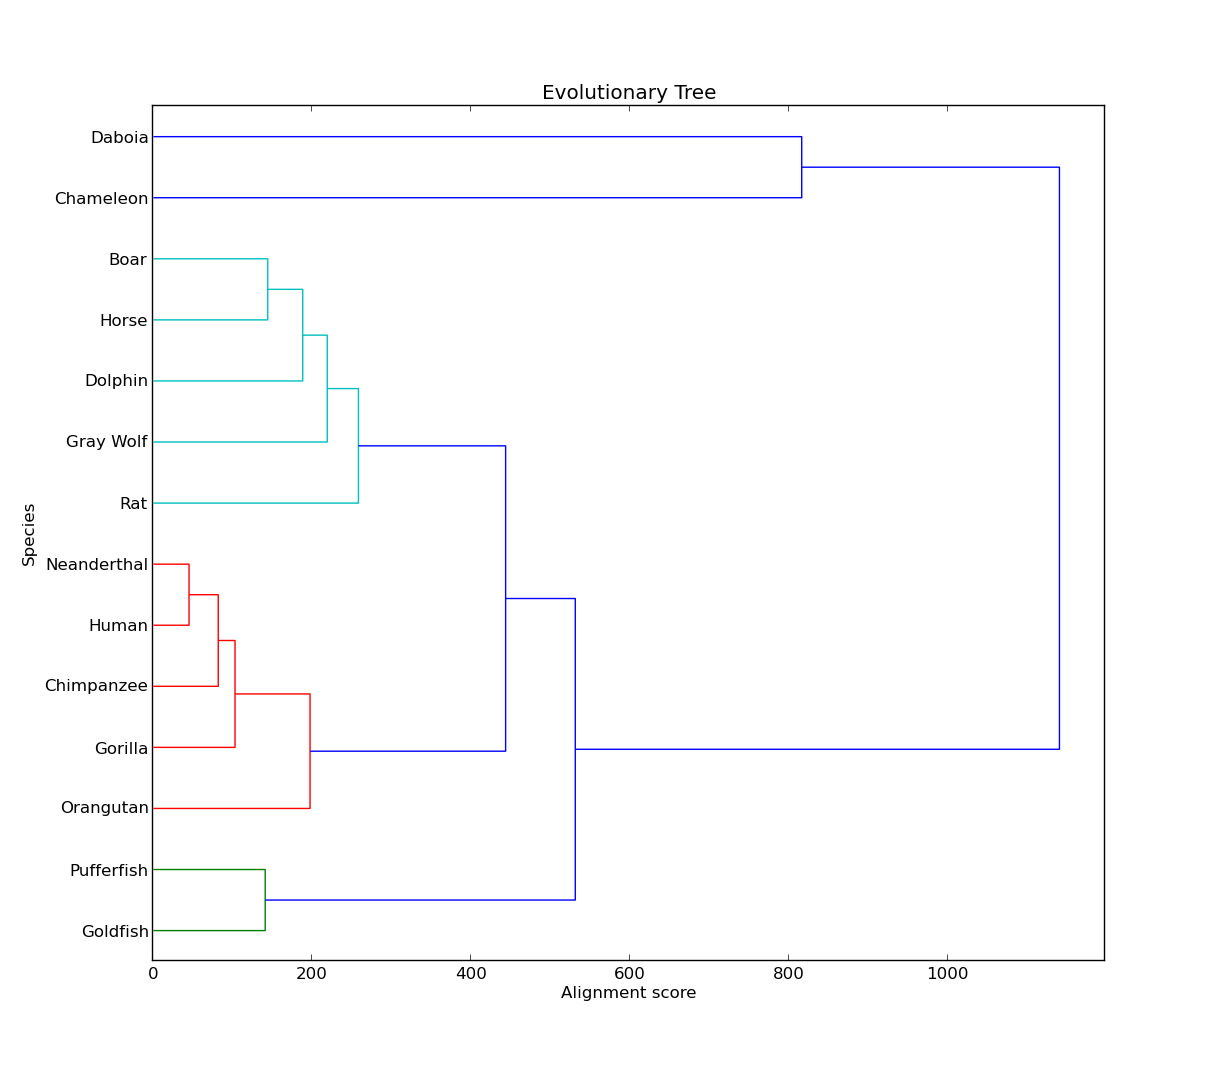
\includegraphics[scale=0.25]{dendro1.png}
\caption{Dendro.}
\label{precrec}
\end{center}
\end{figure}

\section*{Honor Code}

% The following paragraph of your report should be included as is - do % not change it.

My answers to homework are my own work. I did not make solutions or code available to anyone else. I did not engage in any other activities that will dishonestly improve my results or dishonestly improve/hurt the results of others.

\end{document}